% Created 2021-02-04 jue 13:32
% Intended LaTeX compiler: pdflatex
\documentclass[presentation,aspectratio=169]{beamer}
\usepackage[utf8]{inputenc}
\usepackage[T1]{fontenc}
\usepackage{graphicx}
\usepackage{grffile}
\usepackage{longtable}
\usepackage{wrapfig}
\usepackage{rotating}
\usepackage[normalem]{ulem}
\usepackage{amsmath}
\usepackage{textcomp}
\usepackage{amssymb}
\usepackage{capt-of}
\usepackage{hyperref}
\usepackage{khpreamble}
\usepackage{amssymb}
\usepgfplotslibrary{groupplots}
\newcommand*{\shift}{\operatorname{q}}
\usetheme{default}
\author{Kjartan Halvorsen}
\date{2021-02-08}
\title{Análisis de elementos de la mecatrónica}
\hypersetup{
 pdfauthor={Kjartan Halvorsen},
 pdftitle={Análisis de elementos de la mecatrónica},
 pdfkeywords={},
 pdfsubject={},
 pdfcreator={Emacs 26.3 (Org mode 9.4.4)}, 
 pdflang={English}}
\begin{document}

\maketitle

\section{Presentación}
\label{sec:org24eebae}
\begin{frame}[label={sec:org7337614}]{¿Quién soy yo}
\begin{center}
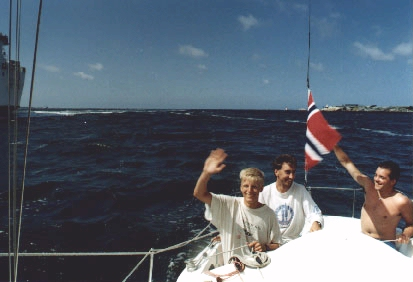
\includegraphics[height=0.6\textheight]{../../figures/red-heat-2.jpeg}
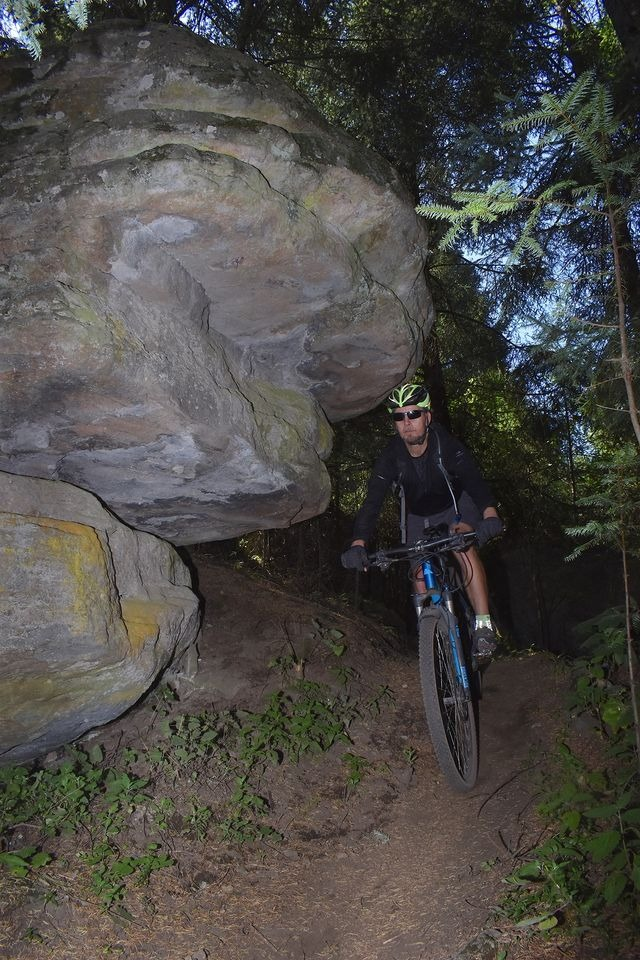
\includegraphics[height=0.6\textheight]{../../figures/mtb.jpeg}
\end{center}
\end{frame}



\begin{frame}[label={sec:org55179bd}]{¿Quién eres tú?}
\end{frame}


\section{Intro}
\label{sec:orga5b41e2}
\begin{frame}[label={sec:org86b4e7b}]{Objetivos, contenido, evaluación}
\end{frame}


\section{Sistemas mecatrónicos}
\label{sec:orge6612b7}

\begin{frame}[label={sec:orgd1cc3b9}]{Sistemas mecatrónicos}
\end{frame}

\begin{frame}[label={sec:org3632ace}]{Eso \alert{no} es un yate ni un sistema mecatrónico}
\begin{center}
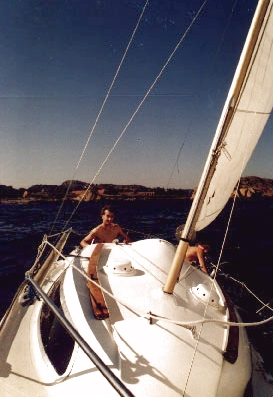
\includegraphics[height=0.6\textheight]{../../figures/red-heat-1.jpeg}
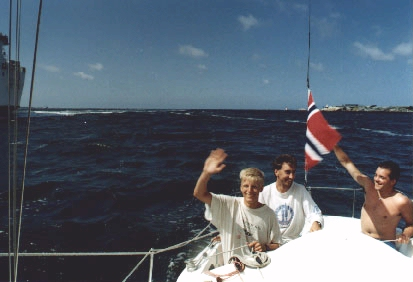
\includegraphics[height=0.6\textheight]{../../figures/red-heat-2.jpeg}
\end{center}
\end{frame}

\begin{frame}[label={sec:org04de5c1}]{Eso \alert{sí} es un yate \alert{y} un sistema mecatrónico}
\begin{center}
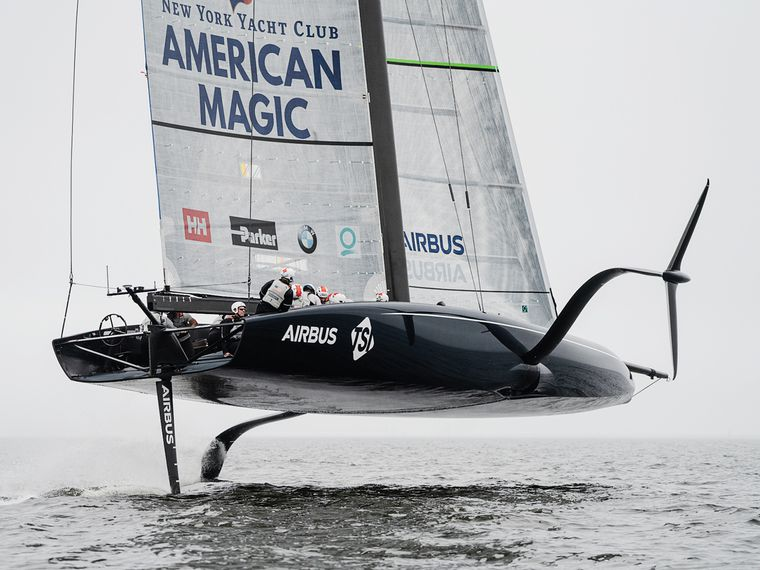
\includegraphics[height=0.7\textheight]{../../figures/ac75.jpeg}\\
{\footnotesize  From SailingWorld}
\end{center}

\href{https://www.sailingscuttlebutt.com/wp-content/uploads/2018/03/AC75\_Class\_Rule.pdf}{AC75 Class rule}
\end{frame}
\begin{frame}[label={sec:org73fb350}]{Videos}
\url{https://youtu.be/VQUl\_hf6yo8}

\url{https://youtu.be/pDn3JVnw\_EI}

\url{https://youtu.be/\_B37zmJpBv4}
\end{frame}

\begin{frame}[label={sec:org8733a51}]{Sistema de hidroalas}
 \begin{center}
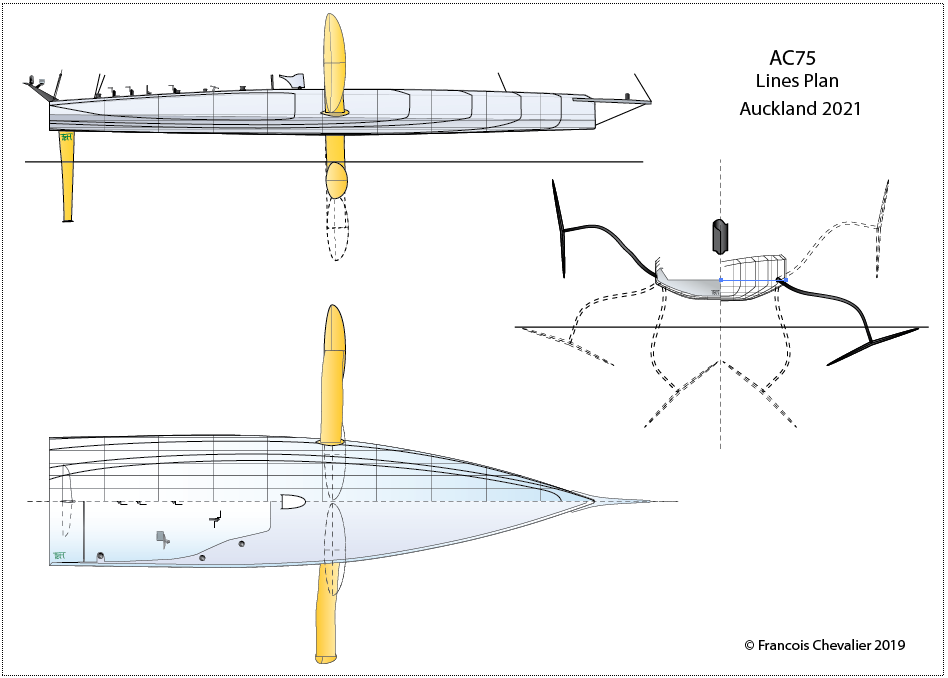
\includegraphics[height=0.6\textheight]{../../figures/AC75-lines.png}
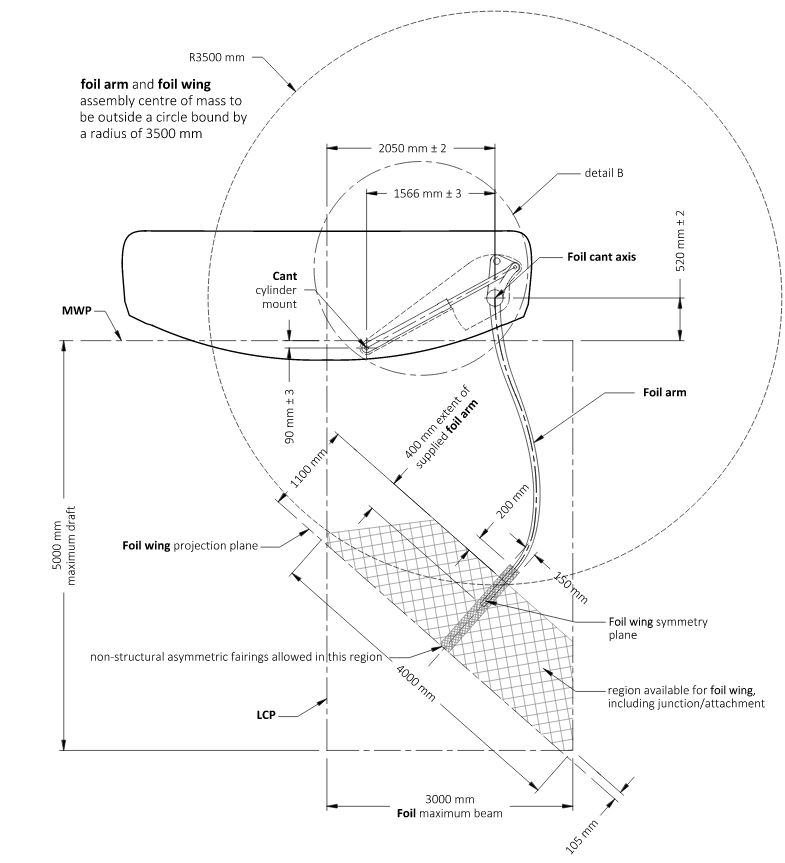
\includegraphics[height=0.7\textheight]{../../figures/AC75-class-foil.png}\\
{\footnotesize  By François Chevalier \hfill From the AC75 Class Rule}
\end{center}
\end{frame}


\begin{frame}[label={sec:org254a290}]{Sistema de hidroalas}
\begin{columns}
\begin{column}{0.5\columnwidth}
\begin{center}
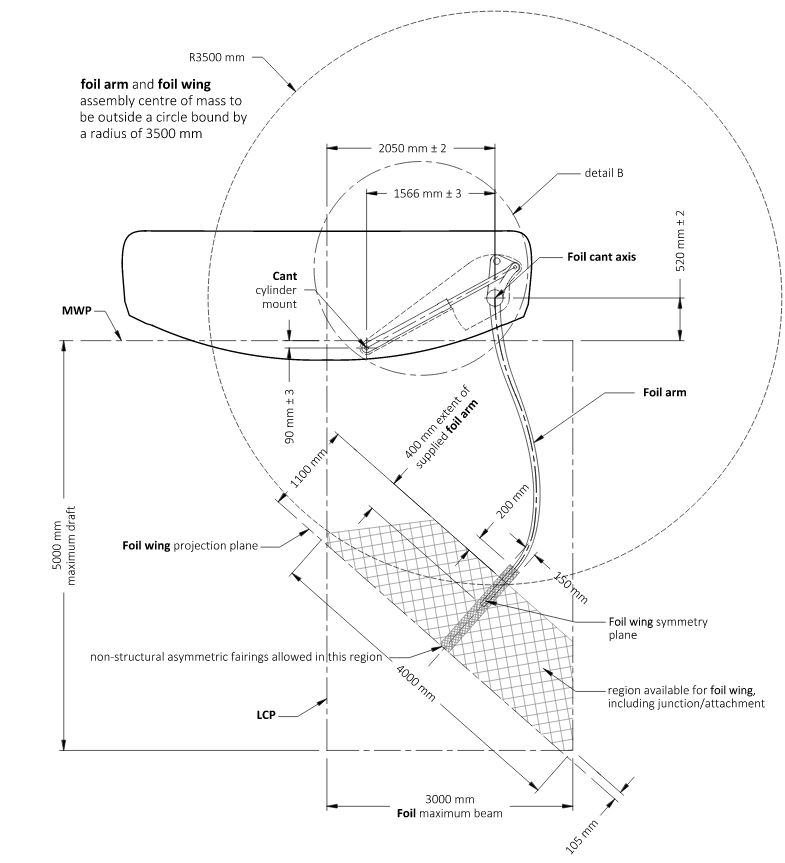
\includegraphics[height=0.8\textheight]{../../figures/AC75-class-foil.png}
\end{center}

{\footnotesize From the AC75 Class Rule}
\end{column}
\begin{column}{0.5\columnwidth}
\begin{itemize}
\item Displacamiento (masa total) - 7.6 t
\item Masa de cada ala - 1.2 t
\item Altura del mástil - 28m
\item Área de vela - 235 sqm
\item Profundidad máxima con alas - 5m
\end{itemize}
\end{column}
\end{columns}
\end{frame}

\begin{frame}[label={sec:orgddd4473}]{Requisitos del sistema mecatrónico de hidroalas}
\begin{center}
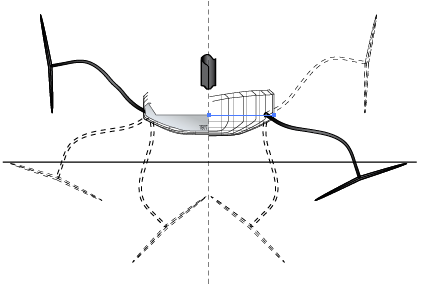
\includegraphics[height=0.3\textheight]{../../figures/AC75-sketch.png}
\end{center}

El sistema debe
\begin{itemize}
\item sústener fuerzas hasta 1000 kN en el ala en posición fija.
\item Poder mover la posición de la ala en un rango de 50 grados en menos de 3 segundos.
\item Poder mover los alerones de las alas.
\item Poder mover los alerones del timón.
\end{itemize}
\end{frame}


\begin{frame}[label={sec:org508a29f}]{Sistema de hidroalas - Actuadores}

\begin{center}
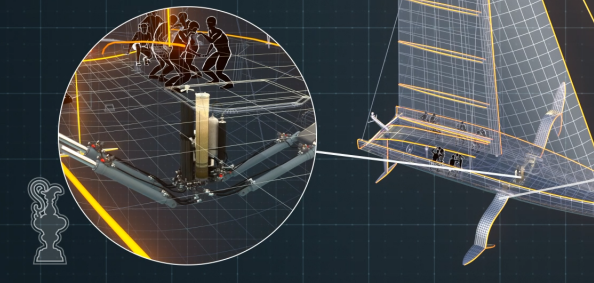
\includegraphics[height=0.4\textheight]{../../figures/AC75-actuators.png}
\end{center}

Actuadores hidraulicos con bomba electrica
\end{frame}

\begin{frame}[label={sec:org927af33}]{Sistema de hidroalas - Sensores}
\begin{itemize}
\item Presión hydraulica
\item \emph{State of Charge} de las pilas
\item Posición continua de los pistones
\item Posición continua de los alereones
\end{itemize}
\end{frame}



\begin{frame}[label={sec:org00af097}]{Sistema de hidroalas - Control}
\begin{itemize}
\item \alert{Feed-forward} Regla 20.1 \emph{No part of a control system may be capable of using feedback from the yacht state to control a control surface}
\item Control de la presión hydraulica
\item Control de posición de los alereones
\item Control de posición de los alereones
\end{itemize}
\end{frame}
\end{document}